\documentclass[a4paper,11pt,oneside]{article}

\usepackage{times}
\usepackage{parskip}
\usepackage{tikz}
\usetikzlibrary{calc,shadows,shapes,backgrounds,patterns,arrows,snakes}
\usepackage{graphicx}
\usepackage[pdftex]{hyperref}
\usepackage[section]{placeins}
\pdfadjustspacing=1

\newcommand{\myname}{Radu Hambasan}
\newcommand{\mytitle}{Faceted Search for Mathematics}
\newcommand{\mysupervisor}{Prof. Michael Kohlhase}

\hypersetup{
  pdfauthor = {\myname},
  pdftitle = {\mytitle},
  pdfkeywords = {},
  colorlinks = {true},
  linkcolor = {blue}
}

\bibliographystyle{unsrt}

\usepackage{paralist}
\usepackage{calbf}
\usepackage{lstomdoc}
\lstset{basicstyle=\sf}
\usepackage[show]{ed}

\def\red#1{\textcolor{red}{#1}}
\def\MWS{\textsf{MWS}\xspace}

\usepackage{wrapfig}
\usepackage{amsfonts}
\usepackage{amsmath}
\usepackage{hyperref}
\newtheorem{definition}{Definition}
\usepackage{xspace}

\usepackage[backend=biber]{biblatex}
\addbibresource{kwarcpubs.bib}
\addbibresource{extpubs.bib}
\addbibresource{kwarccrossrefs.bib}
\addbibresource{extcrossrefs.bib}
\addbibresource{rest.bib}

\usepackage{listings}

\usepackage{bera}
\usepackage{listings}
\usepackage{xcolor}

\colorlet{punct}{red!60!black}
\definecolor{background}{HTML}{EEEEEE}
\definecolor{delim}{RGB}{20,105,176}
\colorlet{numb}{magenta!60!black}
\lstdefinelanguage[m]{MathML}[]{XML}{keywordsprefix={m:},sensitive=true}
\lstdefinelanguage[mws]{MWS}[]{XML}{keywordsprefix={mws:},sensitive=true}
\lstdefinelanguage{json}{
    basicstyle=\normalfont\ttfamily,
    numbers=left,
    numberstyle=\scriptsize,
    stepnumber=1,
    numbersep=8pt,
    showstringspaces=false,
    breaklines=true,
    frame=lines,
    backgroundcolor=\color{background},
    literate=
     *{0}{{{\color{numb}0}}}{1}
      {1}{{{\color{numb}1}}}{1}
      {2}{{{\color{numb}2}}}{1}
      {3}{{{\color{numb}3}}}{1}
      {4}{{{\color{numb}4}}}{1}
      {5}{{{\color{numb}5}}}{1}
      {6}{{{\color{numb}6}}}{1}
      {7}{{{\color{numb}7}}}{1}
      {8}{{{\color{numb}8}}}{1}
      {9}{{{\color{numb}9}}}{1}
      {:}{{{\color{punct}{:}}}}{1}
      {,}{{{\color{punct}{,}}}}{1}
      {\{}{{{\color{delim}{\{}}}}{1}
      {\}}{{{\color{delim}{\}}}}}{1}
      {[}{{{\color{delim}{[}}}}{1}
      {]}{{{\color{delim}{]}}}}{1},
}

\def\cS{\mathcal{S}}
\let\phi=\varphi\let\tilde=\widetilde
\def\mws{\textsf{MathWebSearch}\xspace}
\def\tms{\textsf{TeMaSearch}\xspace}
\def\els{\textsf{Elasticsearch}\xspace}
\def\cmml{\textsf{Content MathML}\xspace}
\def\pmml{\textsf{Presentation MathML}\xspace}
\def\xml{\textsf{XML}\xspace}
\def\xhtml{\textsf{XHTML}\xspace}
\def\xpath{\textsf{XPath}\xspace}
\def\arxiv{\textsf{ArXiv}\xspace}
\def\latexml{\LaTeX{ML}\xspace}
\def\arxmliv{\textsf{ArXMLiv}\xspace}
\def\mathml{\textsf{MathML}\xspace}
\def\zblatt{\textsf{Zentralblatt}\xspace}
\def\latex{\LaTeX}
\def\tex{\TeX}

\bibliography{kwarc,rest}

\begin{document}
\pagenumbering{roman}

\thispagestyle{empty}

\begin{flushright}
    
\includegraphics[scale=0.7]{img/jub-logo}
\end{flushright}
\vspace{20mm}
\begin{center}
    \huge
    \textbf{\mytitle}
\end{center}
\vspace*{4mm}
\begin{center}
    \Large by
\end{center}
\vspace*{4mm}
\begin{center}
    \Large
    \textbf{\myname}
\end{center}
\vspace*{20mm}
\begin{center}
    \large
    Bachelor Thesis in Computer Science
\end{center}
\vfill
\begin{flushright}
    \large
    \begin{tabular}{c}
        \mysupervisor \\
        \hline
        Supervisor \\
        \\
    \end{tabular}
\end{flushright}
\vspace*{8mm}
\begin{flushleft}
    \large
    Date of Submission: \today \\
    \rule{\textwidth}{1pt}
\end{flushleft}
\begin{center}
    \Large Jacobs University --- School of Engineering and Science
\end{center}

\newpage
\thispagestyle{empty}

With my signature, I certify that this thesis has been written by me using
only the indicated resources and materials. Where I have presented data and
results, the data and results are complete, genuine, and have been obtained by
me unless otherwise acknowledged; where my results derive from computer
programs, these computer programs have been written by me unless otherwise
acknowledged. I further confirm that this thesis has not been submitted, either
in part or as a whole, for any other academic degree at this or another
institution.

\vspace{20mm}

Radu Hambasan \hfill Bremen, \today

\newpage

\section*{Abstract}
Faceted search represents one of the most practical ways to browse a large
corpus of information. Information is categorized automatically for
a given query and the user is given the opportunity to further refine
his/her query. Many search engines offer a powerful faceted search engine,
but only on the textual level. Faceted Search in the context of Math Search
is still unexplored territory.

In this thesis, I describe one way of solving the faceted search problem in
math: by extracting recognizable formula schemata from a given set of formulae
and using these schemata to divide the initial set into formula classes. Also,
I provide a direct application by integrating this solution with existing
services.

\tableofcontents

\clearpage \pagenumbering{arabic}

\section{Introduction}\label{sec:intro}

The size of digital data has been growing tremendously since the invention
of the Internet. Today, the ability to quickly search for relevant information
in the vast amount of knowledge available is essential in all domains.
As a consequence, search engines have become the prevalent tool for exploring
digital data.

Although text search engines (e.g. Google~\cite{google:online} or
Bing~\cite{bing:online}) seem to be successful for the average user, they are
limited when it comes to finding scientific content. This is because
STEM\footnote{Science, Technology, Engineering and Mathematics} documents are
mostly relevant for the mathematical formulae they contain and math cannot be
properly indexed by a textual search engine, because the hierarchical structure
of the content is also important.

A good math search engine is therefore needed in several applications.
For example, a large airline may have many ongoing research projects and could
significantly improve efficiency if they had a way of searching for formulae in
a corpus containing all their previous work. The same holds for all large
physics-oriented research centers, such as CERN. Valuable time would be saved
if scientists would have a fast, reliable and powerful math search engine to
analyse previous related work. As a third application, university students
should be mentioned. Their homework, research and overall study process would
be facilitated once they are provided with more than textual search. For all
these applications, we need first a strong math search engine and second a
large corpus of math to index.

The Cornell e-Print Archive, \arxiv, is an example of such a corpus, containing
over a million STEM documents from various scientific fields (Physics,
Mathematics, Computer Science, Quantitative Biology, Quantitative Finance and
Statistics)~\cite{arXiv:online}. Having almost a million documents, with
possibly more than a billion formulae, the search engine must provide an
expressive query language and query-refining options to be able to retrieve
useful information. One service that provides both these is the Zentralblatt
Math service~\cite{zbmath:online}.

Zentralblatt Math now employs formula search for access to mathematical
reviews~\cite{KohMihSperTes:mfs13}. Their database contains over 3 million
abstract reviews spanning all areas of mathematics. To explore this database
they provide a powerful search engine called ``structured search''. This engine
is also capable of faceted search.  Figure~\ref{fig:zbFaceted} shows a typical
situation: a user searched for a keyword (here an author name) and the faceted
search generated links for search refinements (the \textbf{facets}) on the
right. Currently, facets for the primary search dimensions are generated --
authors, journals, MSC, but not for formulae. In this way, the user is given
the ability to further explore the result space, without knowing in advance the
specifics of what he/she is looking for.  Recently, formula search has been
added as a component to the structured search facility. However, there is still
no possibility of faceted search on the math content of the documents.

\begin{figure}[ht]\centering
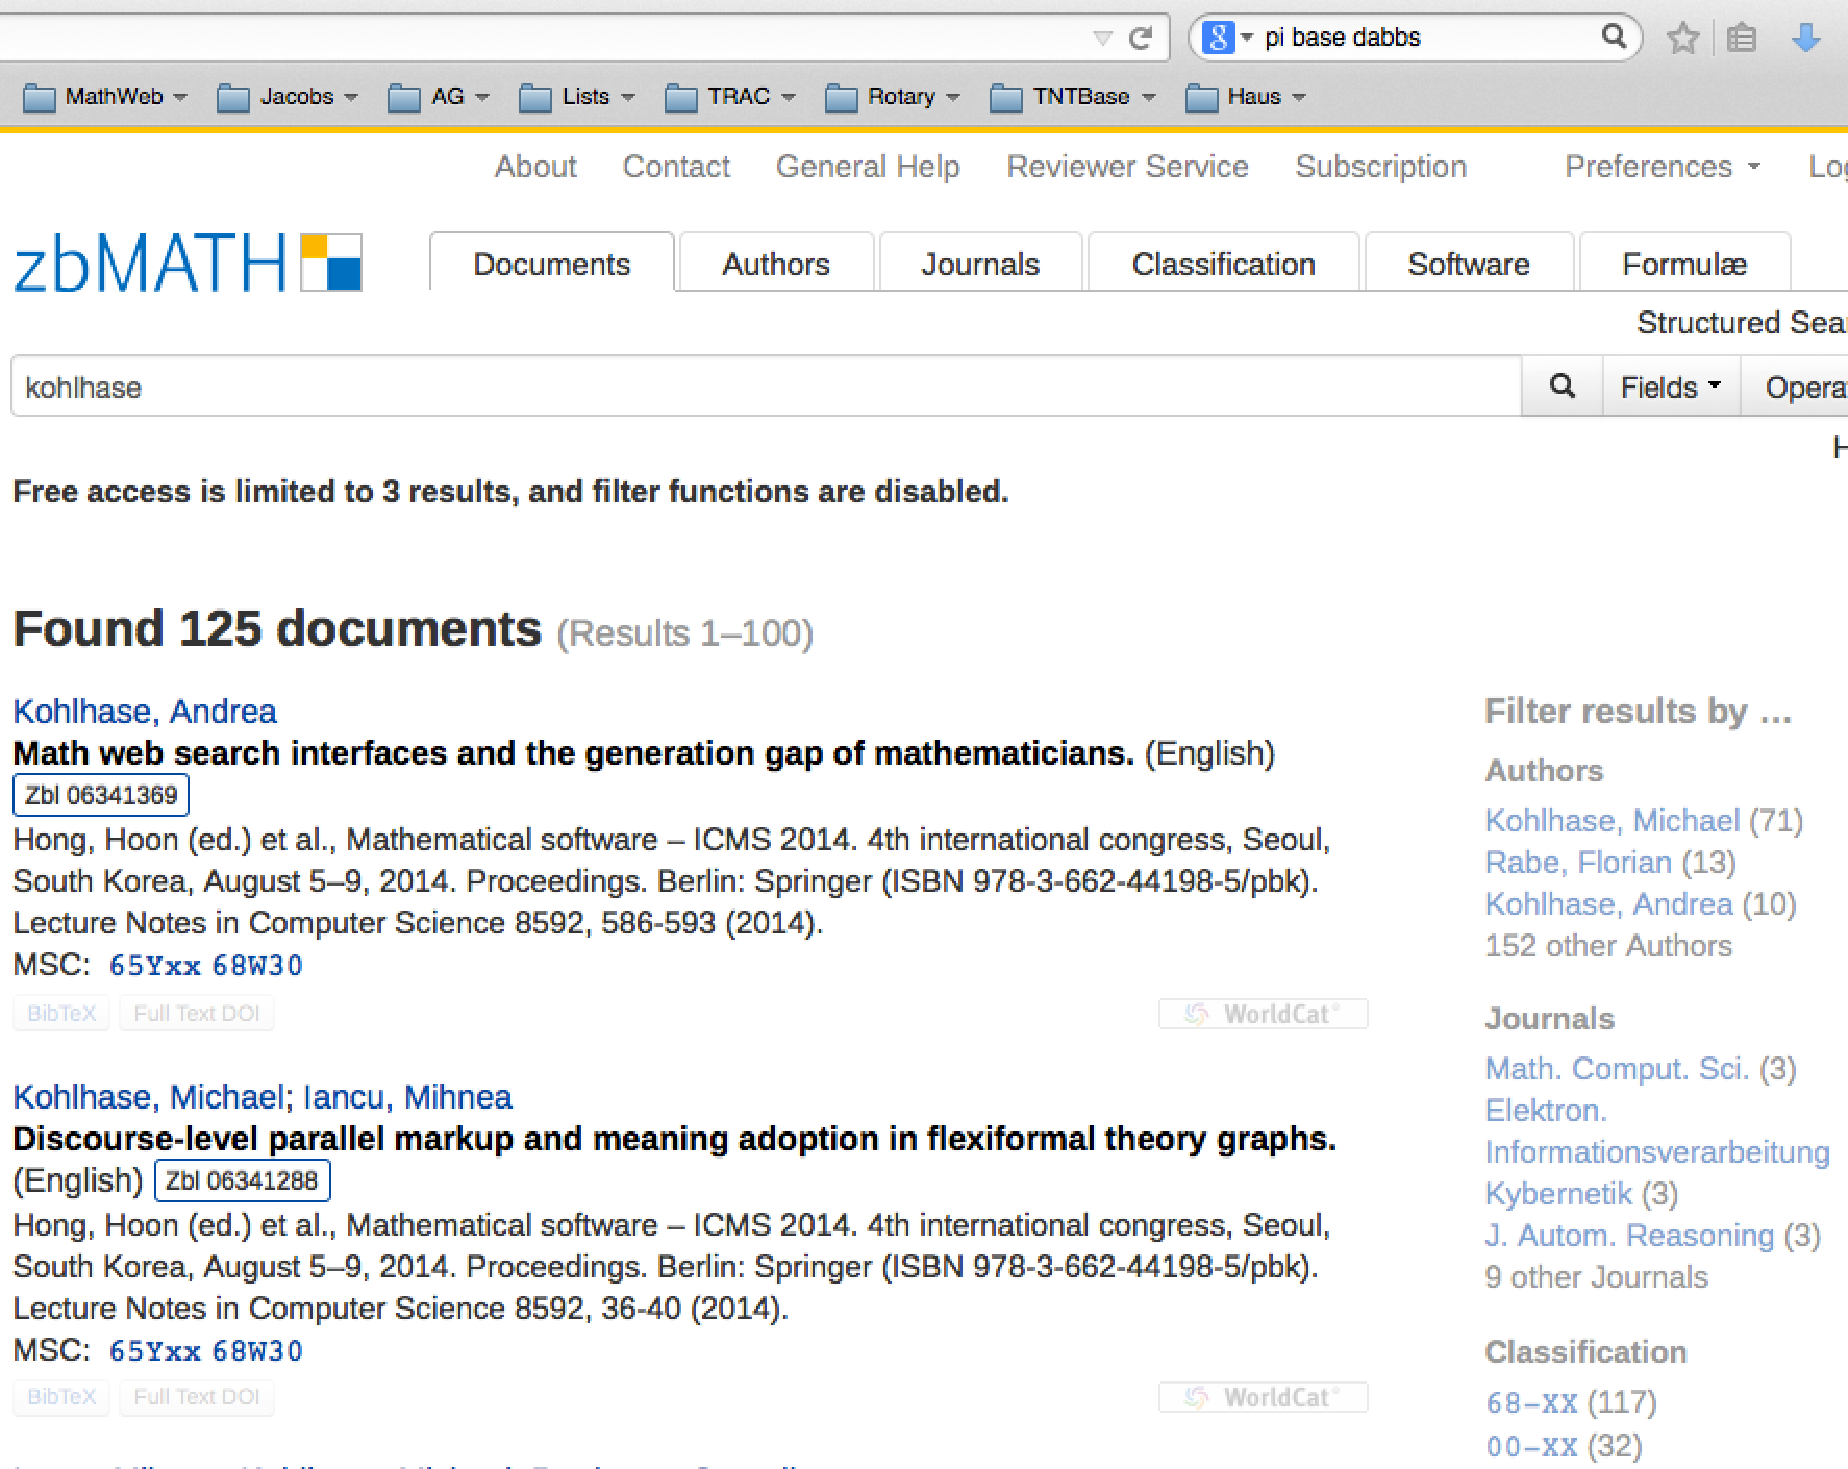
\includegraphics[width=12.7cm]{img/faceted-search.pdf}
\caption{Faceted Search in ZBMath}\label{fig:zbFaceted}
\end{figure}

There are multiple ways in which we could understand a ``math facet''.  One way
would be through the MSC classification~\cite{MSC-SKOS}.  However, this would
be rather vague because it will only provide info about the field of
mathematics to which an article belongs. If the authors use formulae from
another field in their paper, the results will suffer a drop in relevance.

I am attempting to solve this problem by extracting formula schemata from the
query hits as formula facets. A math facet consists of a set of formula
schemata generated to further disambiguate the query by refining it in a new
dimension.  For instance, for the query above we could have the formulae in
Figure~\ref{fig:formula-facets}, which allows the user to drill in on
\begin{inparaenum}[\em i\rm)]
\item variation theory and minimal surfaces,
\item higher-order unification, and
\item type theory.
\end{inparaenum}
Following the \MWS (see~\ref{subsec:prelim:mws}) tradition, the red identifiers
stand for query variables, their presence making the results \textbf{formula
schemata}.

\begin{wrapfigure}r{4.6cm}\vspace*{-1em}
\begin{tabular}{l}
$\int_{\red{M}}{\red\Phi(d_p\red{f}) dvol}$\\[1ex]
$\lambda{\red{X}}.h(H^1\red{X})\cdots{H^n\red{X}}$\\[1ex]
$\frac{\red\Gamma\vdash\red{A}\gg\red\alpha}{\red{D}}$
\end{tabular}\vspace*{-.5em}
\caption{formula facets}\label{fig:formula-facets}\vspace*{-1em}
\end{wrapfigure}

These formula schemata were manually created, but for an application we need to
generate them automatically from the query. Moreover, each schema should
further expand to show the formula class it represents. Formula classes would
consist of all formulae sharing the same schema. This is the algorithmic
problem I explore in the thesis.


\section{Preliminaries}\label{sec:prelim}

In this section we describe the existent systems on which our work will be
based, with the intention of making this thesis self-contained. We will
present these systems in detail in the rest of this section, but
below is a summary of the role they play in our work:
\begin{itemize}
\item \textbf{MathWebSearch} which provides the necessary index structure
for schema search.
\item \textbf{Elasticsearch} which provides hits in response to text query,
    as well as run aggregations on the hits.
    These hits represent formulae to be schematized.
\item \textbf{arXiv} which provides a large corpus of mathematical documents
    that we can index and run our system on.
\item \textbf{\latexml} which converts \latex expressions to MathML.
\end{itemize}

\subsection{Project Goals}\label{subsec:prelim:goals}
As discussed in Section~\ref{sec:intro}, the goal of this project is to
develop a scalable formula schematization engine, capable of dividing a set of
query hits into classes, according to the generated formula schemata.

We have set the following end-user requirement for our system:
\begin{enumerate}
    \item it should be able to generate formula schemata from a
        given set of formulae and the resulting schemata should be easily
        recognizable by the user.
    \item it should be able to classify the given set of formulae according to
        the generated schemata.
    \item the system should be massively scalable, i.e. capable of answering
        queries with hundreds of thousands of formulae in a matter of seconds.
\end{enumerate}

\subsection{MathWebSearch}\label{subsec:prelim:mws}

At its core, the \mws system (MWS) is a content-based search engine for
mathematical formulae. It indexes MathML formulae, using a technique derived
from automated theorem proving: Substitution Tree Indexing.
Recently, it was augmented with full-text search capabilities, combining
keywords query with unification-based formula search. The engine serving
text queries is \els~\ref{subsec:prelim:els}.
From now on, in order to avoid confusion, we will refer to the core system
(providing just formula query capability) as \MWS and to the complete service
(\MWS + \els) as \tms.

The overall workflow of \tms is the following:
\begin{enumerate}
    \item HTML5 documents representing mathematical articles are
        crawled to generate \MWS harvests~\cite{mwsharvest:online}.
        \textsf{.harvest} is an extension of \mathml which \MWS can index. Its
        role is to separate the math from the text in a given document.
    \item \MWS indexes the harvests.
    \item a second pass is made over the harvests to generate annotated
        documents (see below).
    \item \els indexes the annotated documents.
    \item Everything is now ready for answering queries. When a query is
        issued, \MWS will answer the mathematical part and \els will answer the
        text part.  The results are combined through a
        NodeJS~\cite{nodejs:online} proxy to send a final result set.
\end{enumerate}

Each mathematical expression is encoded as a set of substitutions based
on a depth-first traversal of its \cmml tree.
Furthermore, each tag from the \cmml tree is encoded as a \textsf{TokenID},
to lower the size of the resulting index. The (bijective) mapping is also
stored together with the index and is needed to reconstruct the original
formula. The index itself is an in-memory trie of substitution paths.

For fast retrieval, in the leaves of the substitution tree, \MWS stores
\textsf{FormulaID}s. These are numbers uniquely associated with formulae,
and they are also used to store context and occurrences about the respective
formula. They are stored in a separate LevelDB~\cite{leveldb:online} database.

A simplified sketch of the index is shown in Figure~\ref{fig:algoindex}.

\mws exposes a RESTful HTTP API which accepts \xml queries.
A valid query must obey the \cmml format, potentially augmented with
\emph{qvar} variables which match any subterms.  A \emph{qvar} variable acts as
a wildcard in a query, with the restriction that if two \emph{qvar}s have the
same name, they must be substituted in the same way.

\tms is using both \mws and \els to answer queries.
In order to achieve cooperation between the two systems, annotated documents
are used. These annotated documents contain metadata from the original document
(e.g. URI, title, author, etc.) and a list of \textsf{FormulaID}s that can be
found in that document.

\subsection{Elasticsearch}\label{subsec:prelim:els}
Elasticsearch~\cite{esl:online} is a powerful and efficient full text search
and analytics engine, built on top of Lucene. It can scale massively, because
it partitions data in shards and is also fault tolerant, because it replicates
data.  It indexes schema-free JSON documents and the search engine exposes a
RESTful web interface.  The query is also structured as JSON and supports a
multitude of features via its domain specific language:  nested queries,
filters, ranking, scoring, searching using wildcards/ranges and faceted search.

The faceted search feature\footnote{Faceted search as such is now deprecated in
ES and was replaced by the more powerful ``aggregations''.} is of particular
interest to us.
One way to use this feature is the terms aggregation: a multi-bucket
aggregation, with dynamically built buckets.
We can specify an array field from a document and ask ES to count how many
unique items from the array are there in the whole index.
This list can also be sorted, e.g. most frequently occurring items first.
Additionally, we can also impose a limit on the number of the buckets (items)
for which we want to receive the count.

An ES query which would return the most frequently used formulae (and
subformulae) for ``Pierre Fermat'', is presented in
Listing~\ref{lst:es_agg_query}. The key part is the \emph{aggs} fields. We are
specifying that we want an aggregation called \textit{Formulae} on ``terms''
(i.e. we want bucket counting) and the target of the aggregation is the fields
\emph{ids}.

\begin{lstlisting}[language=json,firstnumber=1,caption=Elastic Search Term
Aggregation Query, captionpos=b, label=lst:es_agg_query]
{
  "query" : {
      "match" : {
          "body" : {
              "query" : "Pierre Fermat",
              "operator" : "and"
          }
      }
  },
  "aggs" : {
      "formulae" : {
          "terms" : { "field" : "ids" }
      }
  }
}
\end{lstlisting}

A possible response to the above query can be found in
Listing~\ref{lst:es_agg_resp}. In the response we can see the returned
aggregations. In our example there is only one and it is called
\emph{formulae}. We can find the actual result in the \emph{buckets} field. The
\textsf{key} field in the bucket corresponds to a \textsf{FormulaID}.
Here, the most frequent formulae were the one with ID 230 and the one with ID
93. The former appeared in 10 documents and the latter appeared in 9 documents.

\begin{lstlisting}[language=json,firstnumber=1,caption=Elastic Search Term
Aggregation Response, captionpos=b, label=lst:es_agg_resp]
{
    ...
    "aggregations" : {
        "formulae" : {
            "buckets" : [
                {
                    "key" : "230",
                    "doc_count" : 10
                },
                {
                    "key" : "93",
                    "doc_count" : 9
                },
                ...
            ]
        }
    }
}
\end{lstlisting}

\subsection{arXiv}\label{subsec:arxiv}
\textbf{arXiv} is a repository of over one million publicly accessible
scientific papers in STEM fields. For the NTCIR-11
challenge~\cite{HamKohPro:man14},
MWS indexed over 8.3 million paragraphs (totaling 176 GB) from arXiv. We will
base our queries on this large index, because it provides a rich database of
highly relevant formulae. Moreover, Elasticsearch will have more formulae on
which it can run aggregations, also leading to more relevant results.

\subsection{\latexml}\label{subsec:latexml}
An overwhelming majority of the digital scientific content is written using
\latex or \tex, due to its usability and popularity among STEM researchers.
However, formulae in these formats are not good candidates for searching
because they do not display the mathematical structure of the underlying
idea. For this purpose, conversion engines have been developed to convert
\latex expressions to more organized formats such as \mathml.

An open source example of such a conversion engine is
\latexml~\cite{Miller:latexml:online}. The \mws project relies heavily on it,
to convert \arxiv documents from \latex to XHTML which is later indexed by \MWS.
It exposes a powerful API, allowing definition files to relate \tex elements to
corresponding XML fragments that should be generated.
For the scope of this project, we will be more interested in another feature of
\latexml: cross-referencing between \pmml and \cmml. While converting \tex
entities to a \pmml tree, each element receives a unique identifier which is
later referenced from the corresponding \cmml element. In this manner, we can
modify the \cmml tree and reflect the changes in the \pmml tree which can be
displayed to the user.


\section{Implementation}\label{sec:implementation}

In this section, I explain the key details of the formula classifier's
implementation, the overall system architecture, as well as the challenges and
trade-offs associated with the taken design decisions.

\subsection{Formalizing the problem}\label{subsec:formal_problem}
Let us now formulate the problem at hand more carefully.

\begin{definition}
  Given a set $\cD$ of documents (fragments) -- e.g. generated by a search
  query, a \textbf{coverage} $0<r\leq1$, and a \textbf{width} $n$, the
  \textbf{Formula Schemata Generation} (FSG) problem requires generating
  a set $\cF$ of at most $n$ formula schemata (content MathML expressions with
  \lstinline|qvar| elements for query variables), such that $\cF$ covers $\cD$.
\end{definition}


\begin{definition}
  We say that a set $\cF$ of formula schemata \textbf{covers} a set $\cD$ of
  document fragments, with \textbf{coverage} $r$, iff at least $r \cdot |\cD|$
  formulae from $\cD$ are an instance $\sigma(f)$ of some $f\in\cF$ for a
  substitution $\sigma$.
\end{definition}

\subsection{An Algorithm for FSG}\label{subsec:fsgAlgorithm}
The FSG algorithm we implemented requires a \MWS index of the corpus.
Given such an index, and a set $\cD$ of formulae (as CMML expressions),
we can find the set $\cF$ in the following way:
\begin{itemize}
    \item Parse the given CMML expressions similarly to \MWS queries,
        to obtain their encoded DFS representations.
    \item Choose a reasonable cutoff heuristic, see~\ref{subsec:cutoffheur}.
    \item Unify each expression with the index, up to a given threshold (given by
        the above heuristic).
    \item Keep a counter for every index path associated with the unifications.
        Since we only match up to a threshold, some formulae will be associated
        with the same path (excluding the leaves).
        We increase the counter each time we find a path already associated
        with a counter.
    \item We sort these path-counter pairs by counter in descending order and
        take the first $n$ ($n$ being the width required by the FSG).
    \item If the threshold depth was smaller than a formula's expression
        depth, the path associated with it will have missing components. We
        replace the missing components with \lstinline|qvar|s to generate the
        schema and return the result set.
\end{itemize}

\begin{wrapfigure}r{5.6cm}\vspace*{-1em}
    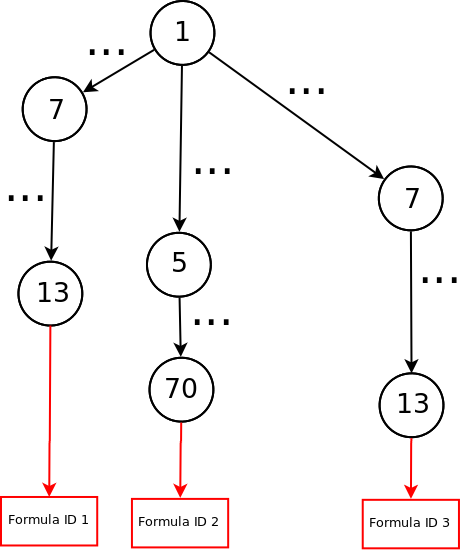
\includegraphics[scale=0.24]{img/FFG_Algo_diag.png}
\caption{Simplified index at depth 1}\label{fig:algoindex}
\end{wrapfigure}

Figure~\ref{fig:algoindex} shows a simplified \MWS index at depth 1.
The formulae's paths represent their depth-first traversal.
Every formula can be reconstructed given its path in the index.
The circles represent index nodes and the number inside represents
the token's ID. When we reach a leaf node, we completely described a
formula. This is encoded in the leaf node by an ID, which can be used
to retrieve the formula from the database.
The length of the arrows symbolizes the depth of the omitted subterms
(for higher depths, we have longer arrows).
Notice how both formula with ID 1 and formula with ID 3 show the same
``path'' when ignoring subterms below a cutoff depth.

\subsection{Finding a cutoff heuristic}\label{subsec:cutoffheur}
In order to generate formula schemata, we must define a ``cutoff heuristic'',
which tells the program when two formulae belong to the same schemata class.
If there was no heuristic, two formulae would belong to the same class,
only if they were identical. However, we want formulae that have something in
common to be grouped together, even if they are not perfectly identical.

One reasonable cutoff heuristic would be a certain expression depth, given as a
parameter to the schema-engine.  In this way, a depth of 0 would always return
$?x$ which corresponds to the 0-unification. The algorithm above is based on
this heuristic.  Another possible choice for the cutoff would be expression
length.  This would output formulae which begin the same way.

\subsection{Design Overview}\label{subsec:design_overview}
The full faceted search system comprises of the following components: the
Formula Schematizer~\ref{subsec:fschematizer}, Elasticsearch, a proxy to
mediate communication between the Schematizer and Elasticsearch and a Web
front-end. The architecture of the system is shown in
Figure~\ref{fig:sys_architecture}.

Once the user enters a query (which consists of keywords and a depth), the
front-end forwards the request to a back-end proxy. The proxy sends the
text component of the query to Elasticsearch and receives back math
contained in matching documents. Afterwards, it sends the retrieved math
and the depth (from the original query) to the Schematizer. The Schematizer
will respond with a classification of the math in formula classes, as well
as the corresponding schema for each class. Finally, the proxy forwards the
result to the front-end which displays it to the user.

In the following sections, I will explain the core components of
the system in detail and describe the challenges faced during
implementation.

\begin{figure}[ht]\centering
    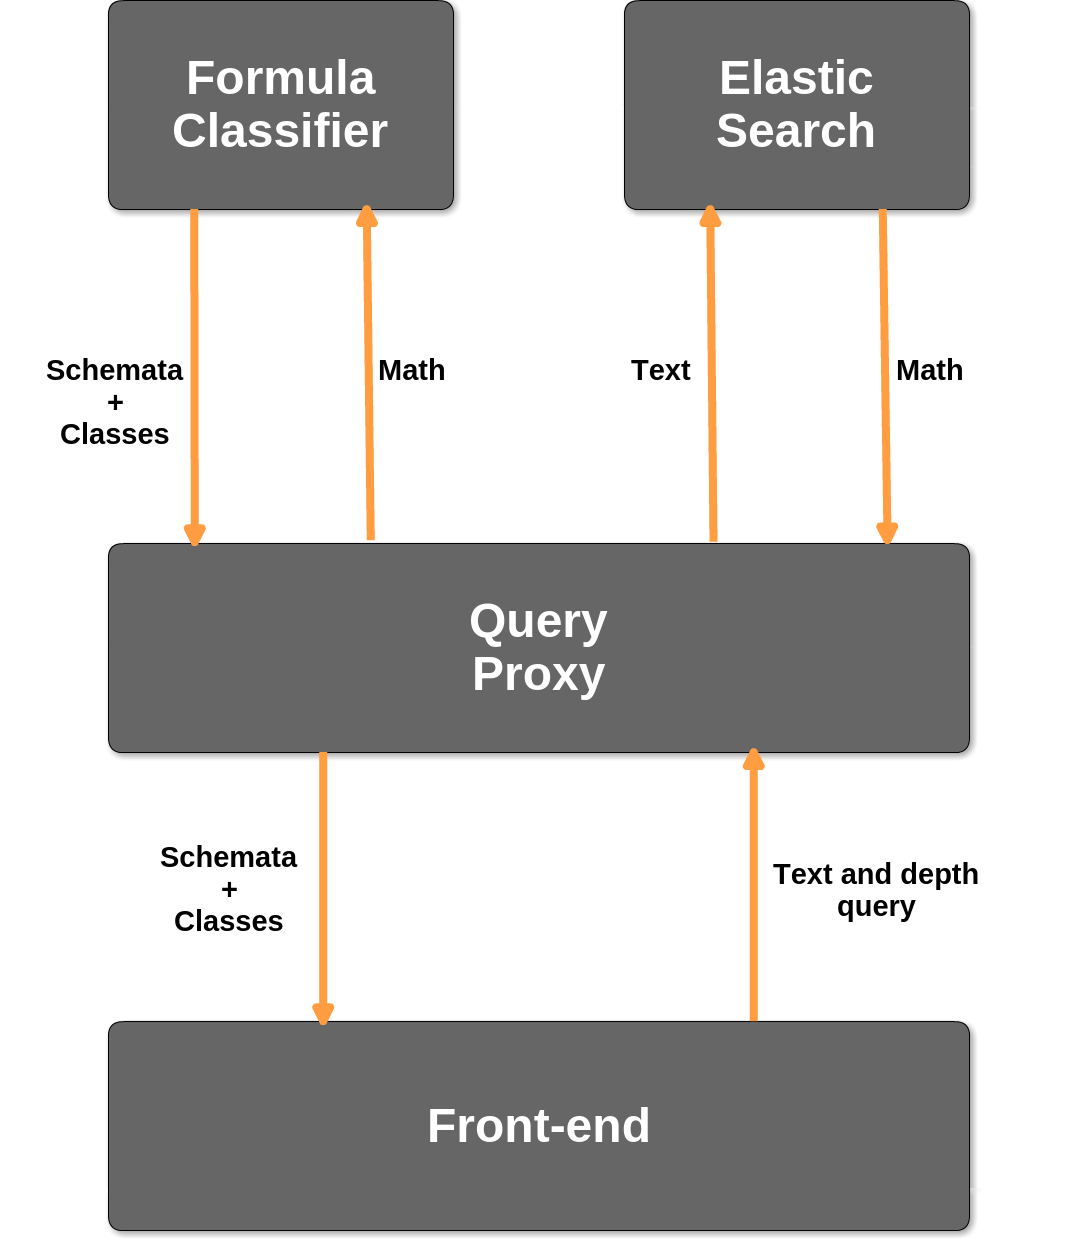
\includegraphics[scale=0.3]{img/SchemaArchitecture.png}
    \caption{Faceted search engine architecture}\label{fig:sys_architecture}
\end{figure}
\FloatBarrier

\subsection{The Formula Schematizer}\label{subsec:fschematizer}
The Schematizer is the central part of our system. It receives a set of
formulae in their \cmml representation, generates corresponding formula
schemata and classifies the formulae according to the generated schemata.
It provides an HTTP endpoint and is therefore self-contained, i.e. it can be
queried independently, not only as part of the faceted search system.
As a consequence, the Schematizer displays a high degree of versatility,
and can be integrated seamlessly with other applications.

Although the algorithm described in Section~\ref{subsec:fsgAlgorithm} works
well in theory, we needed to adapt it considering various \mws implementation
details, e.g. the index is read-only (therefore we cannot store extra data into
the index nodes). Therefore, the overall idea/theory is the same, but now we take the
following shortcut: instead of unifying every formula with the index, we just
pretend we do and instead generate a ``signature'' for each formula. This
signature is the path shown in Section~\ref{subsec:fsgAlgorithm}. We use the
\mws encoding for \mathml nodes, where each node is assigned an integer ID
based on its tag and text content. If the node is not a leaf, then only the tag
is considered. The signature will be a vector of integer IDs, corresponding to
the pre-order traversal of the \cmml tree.

Naturally, the signature depends on the depth chosen for the cutoff heuristic.
At depth 0, the signature consists only of the root token of the \cmml
expression. At full depth (the maximum depth of the expression), the signature
is the same as the depth-first traversal of the \cmml tree.
\ednote{Add signature examples}

Based on these computed signatures, we divide the input set of formulae into
formula classes, i.e. all formulae with the same signature belong to the same
class. For this operation we keep an in-memory hash table, where the keys are
given by the signatures and the values are sets of formulae which have the
signature key. After filling the hash table, we sort it according to the number
of formulae in a given class, since the signatures which cover the most
formulae should come at the beginning of the reported result.

The Schematizer caller can place a limit on the maximum number of schemata to be
returned. If such a limit was specified, we apply it to our sorted list of
signatures and take only the top ones.

As a last step, we need to construct \cmml trees from the signatures, in order
to be able to show the schemata as formulae to the user. We are able to do
this because we know the arity of each token and the depth used for cutoff.
The tree obtained after the reconstruction might be incomplete, so we insert
query variables in place of missing subtrees.
We finally return these \cmml trees with query variables (the formula
schemata), together with the formulae which they cover.

\subsection{The Elasticsearch proxy}\label{subsec:esproxy}
In order to obtain formulae to feed as input to the Schematizer, we will make
use of Elasticsearch. The corpus indexed by Elasticsearch consists of 176 GB of
\arxiv documents annotated using the format described in
Section~\ref{subsec:prelim:mws}

To mediate the communication between the two components (Elasticsearch and the
Schematizer), a NodeJS proxy was developed. The proxy exposes an HTTP
interface, which will be used by an eventual front-end for querying.
There are three important query parameters: the keywords, the depth and the
maximum schemata count.

The main task of the proxy is to assemble the Elasticsearch JSON query after
receiving the parameters from the front-end and forward the Elasticsearch
results to the Schematizer. To ensure a fast response, only a minimum of
preprocessing is done between the stages.

Once the Schematizer has generated schemata and has classified the formulae,
the proxy assembles the results into a JSON object which it sends to the
front-end.

\subsection{The Front-End}\label{subsec:frontend}
To demonstrate the capabilities of the Schematizer, as well as provide an
access point for the user, a simple front-end was developed.
As shown in figure~\ref{fig:frontend}, the user can enter a set of keywords for
the query, as well as a schema depth, which defaults to 3. The maximum result
size is not accessible to the user, to prevent abuses and reduce server load.

\begin{figure}[ht]\centering
    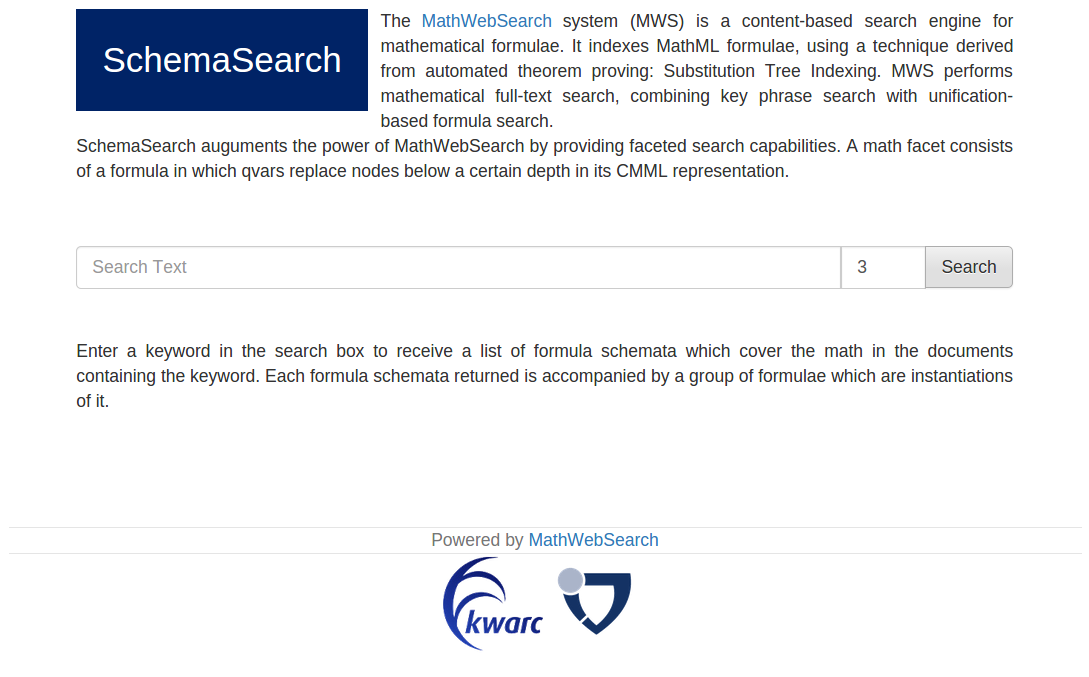
\includegraphics[width=12.8cm]{img/frontend.png}
    \caption{Faceted search front-end}\label{fig:frontend}
\end{figure}
\FloatBarrier

\subsection{ES aggregations}\label{subsec:esagg}
Initially, the ``aggregations'' feature of Elasticsearch seemed to be a
suitable improvement for the Schematizer and the ES script was originally
designed to request math in a term-based aggregation format, as described in
Section~\ref{subsec:prelim:els}. However, on a closer look we can see that not
only are aggregations not needed, but they influence the results in a negative
way.

On a regular query, the top formulae reported using aggregations were trivial
formulae, i.e. consisting of only one or two symbols. This is because authors
frequently use short inline math to refer to their results. As a consequence,
the top returned was completely unusable, because the first hits were
irrelevant. Moreover, it was impossible to distinguish between long irrelevant
expressions and infrequently used important expressions since both of them
ranked the same.

As an added disadvantage of using aggregations, we must mention the time
overhead. For obtaining accurate results over the entire index, several
minutes were needed. In order to reach our target time of \~10s, we had to
drastically shrink down the number of considered aggregations (down to 100).
As mentioned before, all these 100 expressions were trivial.

Given the drawbacks mentioned above, we decided against using aggregations in
the Schematizer pipeline. As an alternative, we will retrieve all math content
from the documents which match the keywords and discard the trivial formulae
using a configurable length heuristic. In practice, this change allowed us to
process more than ten thousand formulae in less than five seconds, which is a
drastic improvement from to the approach using aggregations.

\subsection{Making the schemata recognizable}\label{subsec:make_sch_recog}
As explained in Section~\ref{subsec:fschematizer}, the initial Schematizer
returned formula schemata as \cmml. Naturally, we would need to transform it to
\pmml in order to be able to display it to the user. For this purpose we used
and XSL stylesheet written by David Carlisle~\cite{carlisle:online}. 
Figure~\ref{fig:cmml_display} shows the initial results of the conversion.

\begin{figure}[ht]\centering
    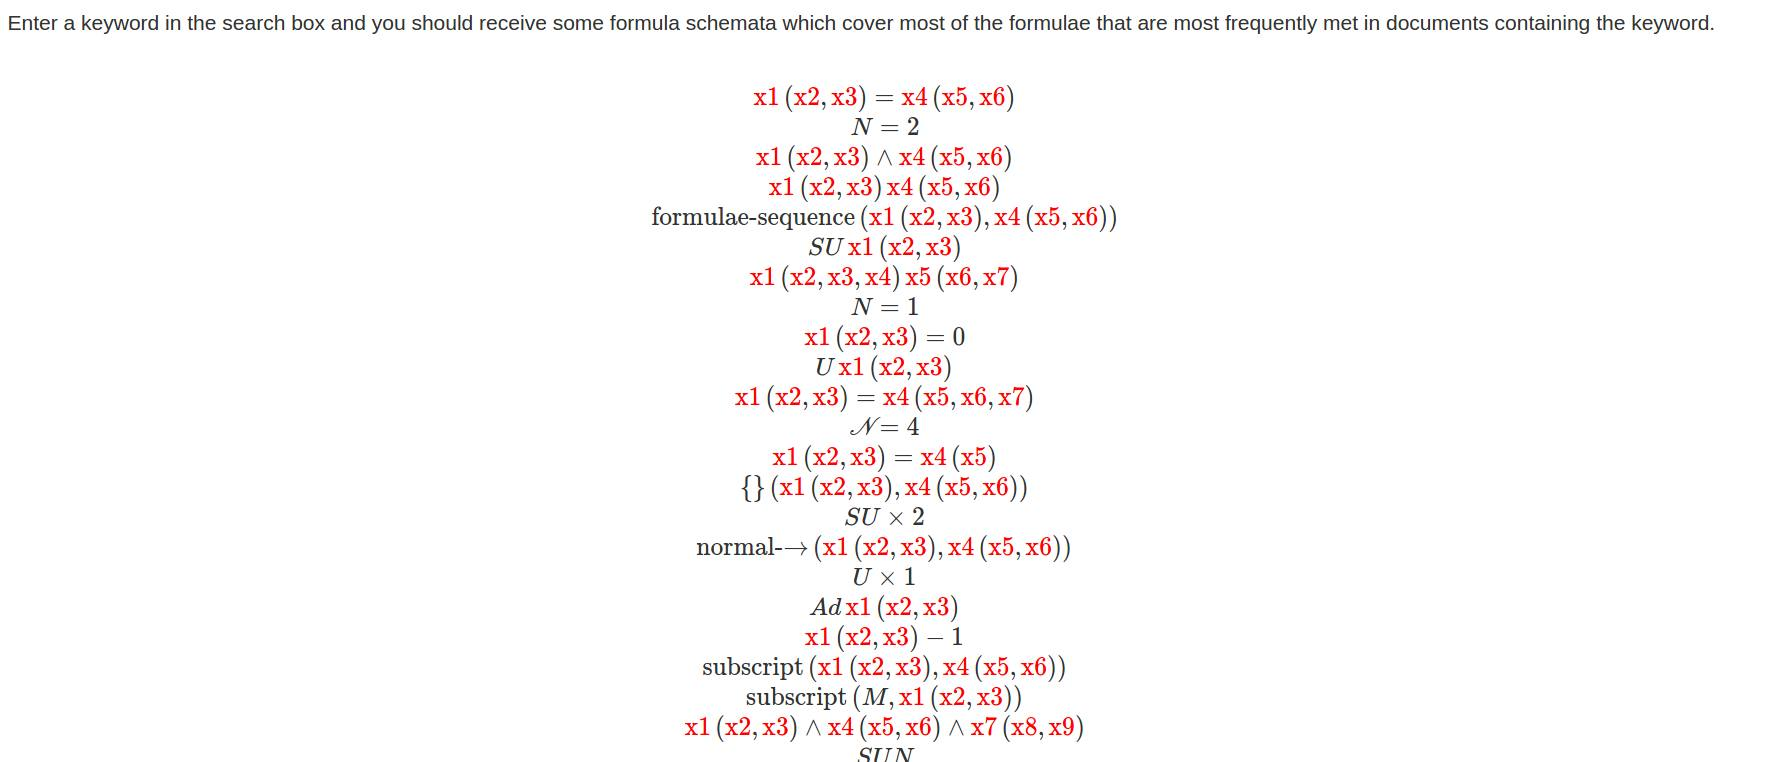
\includegraphics[width=12.8cm]{img/firstAttempt.jpg}
    \caption{Displaying Content MathML}\label{fig:cmml_display}
\end{figure}
\FloatBarrier

It is clear that the conversion leads to somewhat disappointing results.
Firstly, they are not recognizable and secondly, they contain left-over text
such as ``subscript'', ``superscript'', ``normal'', etc.
On a deeper analysis, we can point out two causes for this strange behaviour.

The reason why schemata are hard to recognize is the inherent ambiguity of
CMML. For instance, a \textsf{csymbol} element can be represented in at least
three different ways depending on the notation being used. \ednote{@Michael:
    Deyan told me that there are >3 ways of representing a csymbol. Can you
    give me some real examples?}
Also, the two applications \verb|apply(f, a, b)| and \verb|apply(+, a, b)| are
described similarly by CMML, but represented in a different manner by PMML. If
the Schematizer replaces the tokens \verb|f|, \verb|a| and
\verb|b| with query variables, both the of applications will be displayed as
\verb|?x1(?x2, ?x3)|, even though we would expect \verb|?x1| to be infix
when it represents the plus operator.

The reason for the left-over text is even simpler: the stylesheet does not
implement enough conversion rules, so it is not able to convert
\verb|subscript|, \verb|superscript| and other elements to PMML.

Although this was a significant hindrance for the faceted search engine, we
managed to overcome it by making use of the cross-reference system
provided by \latexml, as discussed in Section~\ref{subsec:latexml}. 
Instead of returning \cmml expressions, the Schematizer will use the first
formula in each class as a template and ``punch holes into
it''\ednote{@Michael: too informal?} effectively returning the ID of the nodes
that are to be substituted with query variables. We will use this IDs to
replace the referenced PMML nodes with \verb|<mi>| nodes representing the
qvars.

The procedure above will solve the left-over text issues, using the template's
initial layout which is valid \pmml. However, we still need to display the
schemata in a way which provides intuition about its class. Heuristically,
we can just keep the first child of apply (the operator) unsubstituted and
replace only the other children (the operands) with query variables.
The results obtained using this heuristic and the cross-reference system are
further discussed in Section~\ref{sec:evaluation}.

\subsection{Naming query variables}\label{subsec:naming_qvars}
As discussed in the section before, we will need a template to modify in order
to display the schema of a class. We are using the first formula as a template,
but any formula in a given class would work as a template for that class.
Since we will process an existing expression, it would be appropriate to name
the query variables in a way which allows the user to perceive some meaning
behind them. For this reason, we conceived a naming convention with the
following rules:

\begin{itemize}
    \item If the node to be replaced is a leaf, its name will be used for the
        qvar.
    \item If the node to be replaced is not a leaf (thus having no name), we
        will use lowercase alphabetical letters from \textsf{a} to \textsf{z}
        preceded by a question mark (according to the \MWS tradition).
    \item If there are more than 26 qvars (thus exceeding the alphabet), we
        name them $x_{1}, x_{2}, \ldots, x_{max\_count}$, also preceded by a
        question mark. This case should be extremely rare.
\end{itemize}

\section{Evaluation}\label{sec:evaluation}
In this section, we will present an evaluation of our faceted search engine.
Firstly, we will examine the front-end (\ref{subsec:fe_results_display}),
obtained after applying the heuristics and improvements described in the
Implementation section. Next, we will analyze the performance of the
Schematizer deployed on an \arxiv index (\ref{subsec:sch_performance}).
In the end, we will look at the API that the Schematizer exposes and elaborate
on its potential (\ref{subsec:schematizer_api}).

\subsection{Front-End results displaying}\label{subsec:fe_results_display}
Figure~\ref{fig:schemata_group} shows the formula schemata at depth 3 for a
query containing the keyword ``Kohlhase''. By default, the top 40 schemata are
shown, but the results are truncated for brevity.
The bold number on the left side of each result item indicates how many
formulae are present in each formula class. For instance, the third schema
represents a formula class containing 10 formulae. The entities marked in red
are query variables (qvars).

\begin{figure}[ht]\centering
    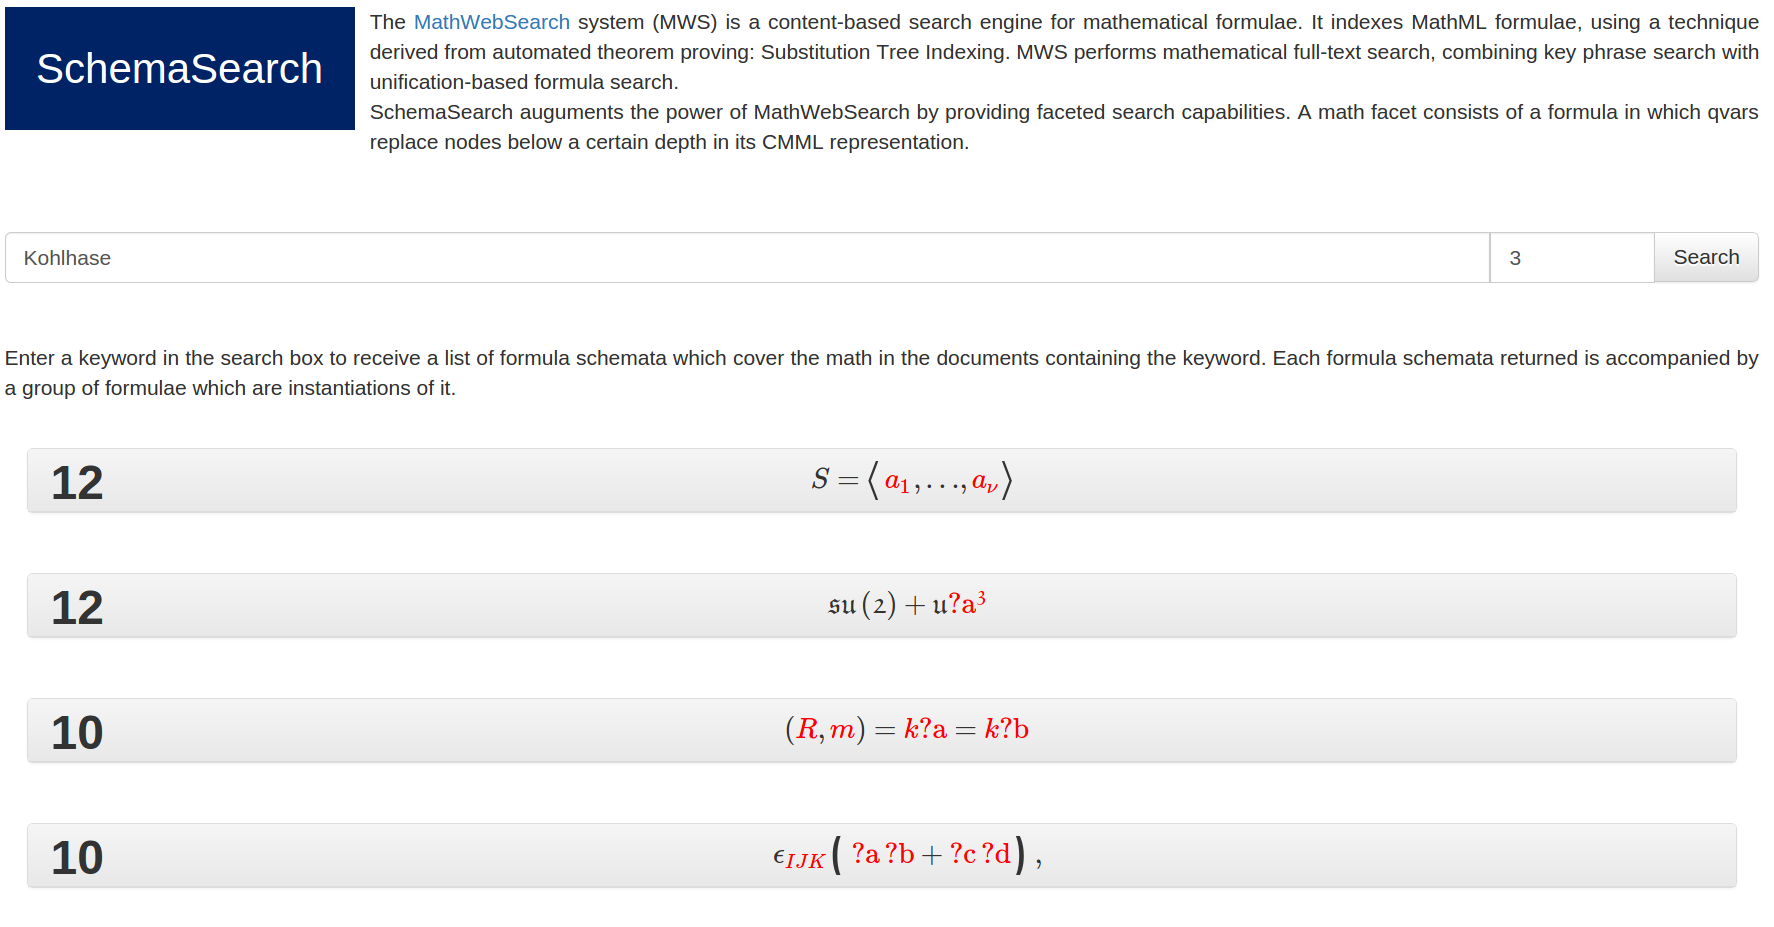
\includegraphics[width=12.8cm]{img/schemataGroup.png}
    \caption{Faceted results at depth 3}\label{fig:schemata_group}
\end{figure}
\FloatBarrier

Figure~\ref{fig:schema_instantiation} shows the expansion of a formula class.
There are three formulae in the class given by this particular math schema, as
indicated by the count on the left upper side. We have one named query
variable, corresponding to a \cmml leaf and 7 anonymous ones marked with
letters from \verb|a| to \verb|g|. 

As explained in Section~\ref{subsec:make_sch_recog}, the first formula from the
class was also used as a template to solve CMML ambiguities. This fact is
easily noticeable by comparing the first formula with the math schema. It is
very intuitive that the former is an instantiation of the latter. We can see
that the named qvar $\red{Z}$ instantiates to $Z$, as expected since it is a
leaf. Other elements from the formula are at a higher depth, so entire
nodes are replaced by the qvars, for example $\red{?b}$ replaces $m^{2}_{R}$.

Despite the close relation between the first member of the class and the
schema, it is slightly less intuitive to see why the other formulae from the
class are instantiations. Between $\red{Z}$ and $\red{?a}$ there is an
invisible times operator. Given the presence of this operator, the left
hand-side of the equality can be expressed in CMML as
\verb|apply(times, Z, ?a)|, which is equivalent to \verb|apply(f, k, 0)|
because all arguments of apply are below the cut-off depth. Since we decided to
keep the first child of apply (the operator) unsubstituted, the left hand-side
might not initially appear as a function application.

A similar issue arises with $\red{?b} + \red{?c}$ and $\frac{1}{\sqrt{W_k}}$.
The user could be under the impression that the former is an addition between
two qvars, when it is actually a function application to two qvars. The
operator of this function application is division for the second formula.
Since both the schema operator (addition) and the formula's operator (division)
are below the cut-off depth, the CMML structure is essentially the same (up to
the cut-off depth).

As we have seen, there is an important trade-off to be made. We can either show
a very cryptic schema which instantiates somewhat more intuitively, or show an
easily recognizable schema with less intuitive instantiations. We have opted
for the second choice, because it seems that the user would be more interested
in receiving relevant schemata as titles for the classes.

\begin{figure}[ht]\centering
    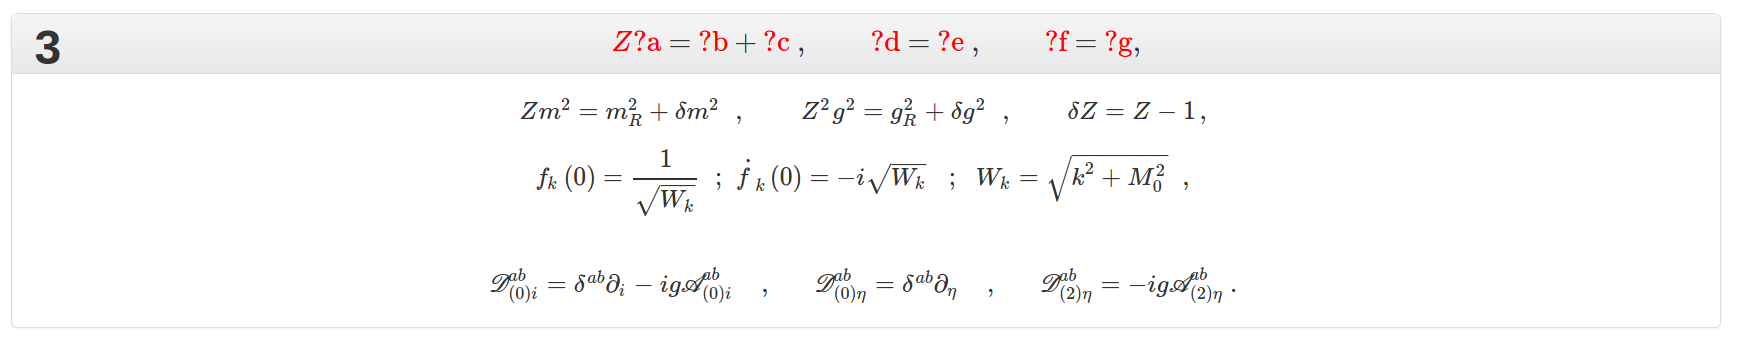
\includegraphics[width=12.8cm]{img/schemaInstantiation.png}
    \caption{Expansion of a formula class}\label{fig:schema_instantiation}
\end{figure}
\FloatBarrier

\subsection{Performance of the Schematizer}\label{subsec:sch_performance}
We designed the Schematizer to be a very lightweight daemon, both as memory
requirements and as CPU usage. To test if we achieved this goal, we benchmarked
it on a server running Linux 3.2.0, with 10 cores (Intel Xeon CPU E5-2650
2.00GHz) and 80 GB of RAM. 

We obtained the 1123 expressions to be schematized by querying Elasticsearch by
the keyword ``Fermat''. While the overall time taken by the faceted search
engine was around 5 seconds, less than a second was spent in the Schematizer.
Also, the CPU utilized by the Schematizer never rose higher than 15\% (as
indicated by the \textsf{top} utility). Asymptotically, the algorithm would run
in $O(N)$ time, where $N$ is the number of input formulae. We are able to reach
linear time performance, because each formula is processed exactly once and the
signature is stored in a hash table, as discussed in
Section~\ref{subsec:fschematizer}.

The space complexity is also linear in the number of formulae, because in the
worst case scenario (large cut-off depth) we will have a schema for every
formula. To analyze the memory footprint of the Schematizer we used
Massif~\cite{massif:online}, a heap profiler from Valgrind's tool suite.
Figure~\ref{fig:heap_usage} shows the total heap memory consumption for a
single query (containing 1123 expressions). Massif reports time using the
number of executed instructions as unit of measurement. The heap memory size is
given in bytes.

There is a short initial steep increase moments after the program started.
This can be attributed to the dynamic linker. Then, the consumption keeps
increasing because we are receiving the formulae (storing them in memory) and
generating the schemata. The peak is reached at 20 MiB, which is impressively
low. Afterwards, there is a sudden decrease in heap size when we drop the
schemata which are not needed (because a \textsf{max\_size} parameter was
specified by the caller). For most of the next part, the heap size stays
constant because we are only processing the signatures and finding the PMML
substitution IDs.

\begin{figure}[ht]\centering
    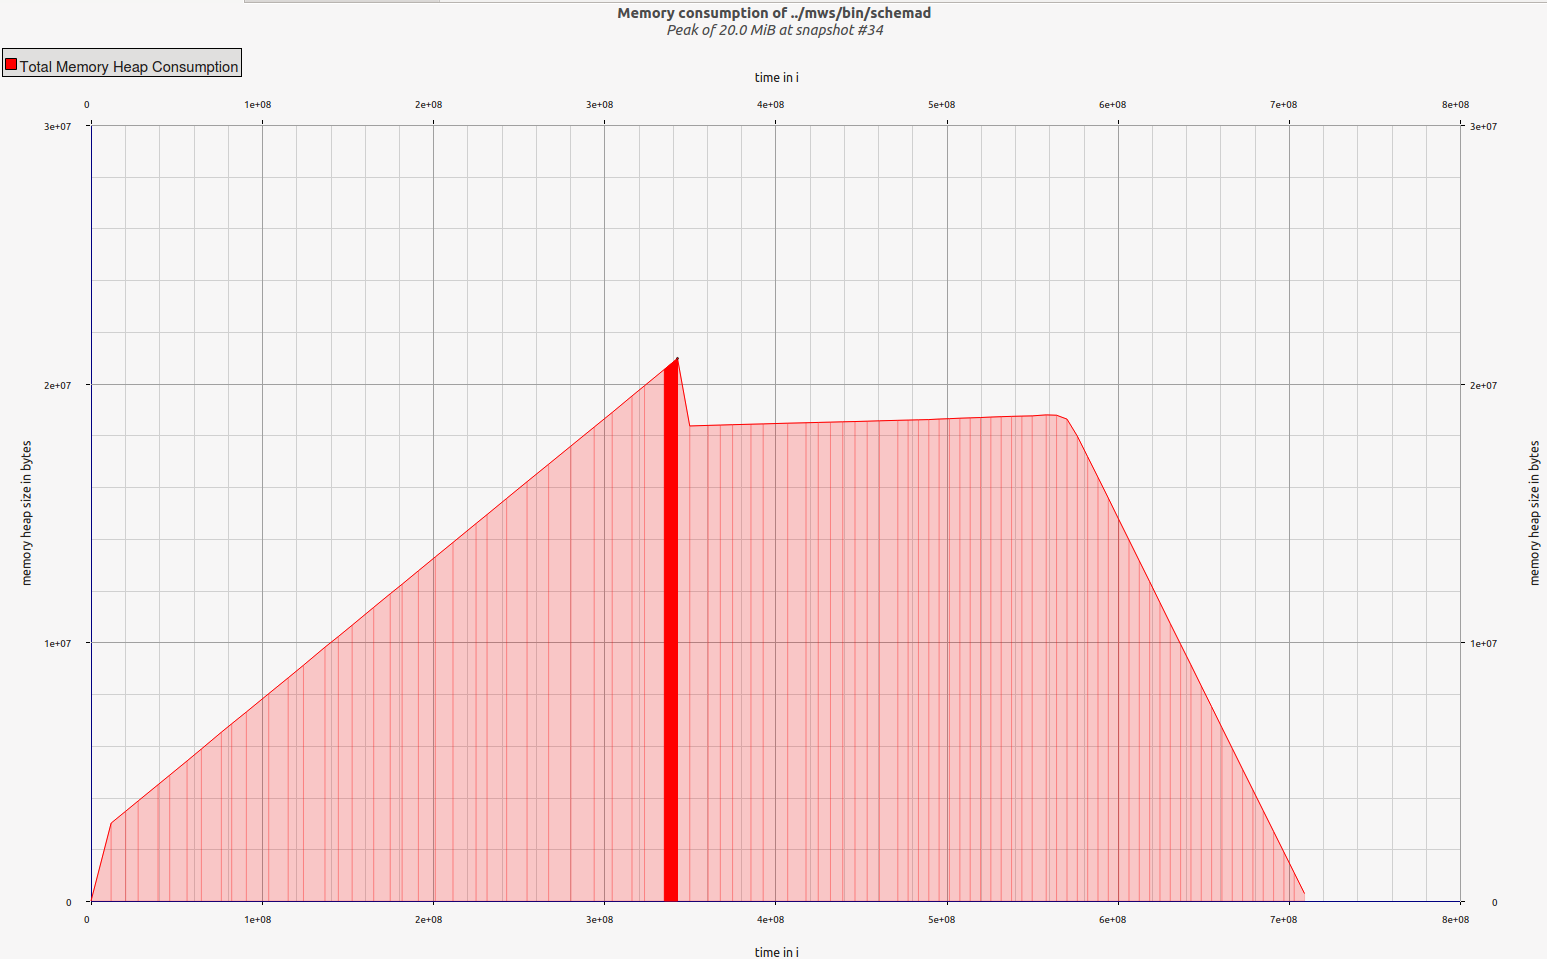
\includegraphics[width=12.8cm]{img/heapUsage.png}
    \caption{Schematizer heap usage for a query}\label{fig:heap_usage}
\end{figure}
\FloatBarrier

All things considered, it is somewhat remarkable that the peak memory usage
is at only 20 MB and only 15\% of one processor is in use for 1123 formulae.
Considering the linear complexity, we can accommodate several millions of
formulae on the mentioned server:
$$80 GB \cdot \frac{1123}{20 MB} \approx 4.5 \cdot {10}^{6} \text{formulae}$$

\subsection{The API}\label{subsec:schematizer_api}
Another relevant point of interest in the Schematizer is its simple, but
sufficient API. By providing an HTTP endpoint, any application which wishes to
use the schematization service can do so, simply by issuing a GET request.
The content of the GET request must be an \xml document, which \verb|mws:query|
as the root element. The children of the \verb|mws:query| are the expressions
to be schematized in \cmml format. The attributes of the query are
\textsf{answsize} (the maximum number of schemata), \textsf{output} (JSON or
XML) and \textsf{depth} (the depth for cut-off).  If JSON is used for the
output, the IDs of PMML substitutions will be returned. If XML is used, formula
schemata in CMML format will be returned.

\section{Conclusion}\label{sec:conclusion}
We have presented the design and implementation of a system capable of
mathematical faceted search. Moreover, we have described a general-purpose
Schematizer which can generate formula schemata and divide expressions into
formula classes according to said schemata. Consequently, we have successfully
addressed all challenges outlined in Section~\ref{subsec:prelim:goals}.

Although the Schematizer provides easily recognizable formulae, some
instantiations might be counterintuitive, which suggests a better cut-off
heuristic is needed. Also, some queries (e.g. using an author as keyword)
provide hits with a very low relevance.  This is because we cannot distinguish
between the work of the author and work where the author is cited at the
textual level. As a consequence, searching for ``Fermat'' would also show
formulae from papers where Fermat was cited and if these papers are numerous,
as it happens with known authors, would provide the user with misleading
results. This suggests that a better source of mathematical expressions might
be required for the Schematizer.

\section{Applications and future work}\label{sec:future}
As we have already noted in the sections before, the most important improvement
we can bring to our faceted search engine is a more relevant source of
formulae. One such source would be \mws. After running a regular \MWS query,
the resulting math hits can be passed to the Schematizer and again divided into
formula classes. This approach would have the advantage of using curated
formulae focused in a specific direction. If the user searches for ``Fermat'',
he might also provide the math query
${\red{?a}}^{\red{?n}} + {\red{?b}}^{\red{?n}}={\red{?c}}^{\red{?n}}$.
By the design of \mws, we would already receive relevant results and we just
need to classify them and use a suitable description (the schema) for the
classes. Moreover, since the query hits must be instantiations of the query,
they would all be structurally similar and hence the relationship between the
hits from a class and the schema will become much more intuitive.

Another improvement angle that can be worked on is the cut-off heuristic. A
good idea might be to use a higher cut-off depth for the first child of apply
(the operator) and a lower cut-off for the other children of apply (the
operands). This would lead to operator leafs being reached faster than other
leafs, which in turn would cause formulae with different operators to separate
into different classes. This should favorably influence the relevance and
appearance of the results since instantiations will become more
recognizable to the user. In our current approach, with a constant cut-off depth,
operators might be treated in the same manner for two formulae, if the cut-off
is too low.

As soon as the relevance of schemata is improved, we can use the faceted search
engine to provide mathematical definitions with the help of
\textsf{NNexus}~\cite{GinCor:nnexus:14}. NNexus is an auto-linker for
mathematical concepts from several encyclopedias, e.g. PlanetMath, Wikipedia.
Assuming we are able to generate relevant schemata in response to keyword
queries, we can target the faceted search engine with all the concepts stored
by NNexus and store a schema for each such concept. Afterwards, for a given
query, we can obtain the schema and check it against our stored set of
schemata. If we find it, we can link the given expression to its mathematical
definition. Given a large number of stored concepts and a high schemata
relevance, the user should be able to see the definition of any encountered
formulae on the web. For example, hovering over $a^2 + b^2 = c^2$ will show the
definition of the Pythagorean theorem.

\printbibliography

\end{document}

